%-------------------------------------------------
\begin{frame}
    \frametitle{Architettura dei Microservizi}
    Ciascun microservizio è stato implementato ispirandosi alla \textbf{Clean Architecture}.

    \smallskip

    \begin{columns}
        \begin{column}{0.5\textwidth}
            \begin{addmargin}[0.6em]{2em}
                In particolare, sono state definiti i seguenti layer:
                \begin{itemize}
                    \item \textbf{Entities}
                    \item \textbf{Use Cases}
                    \item \textbf{Adapters}
                    \item \textbf{Drivers}
                \end{itemize}
            \end{addmargin}
        \end{column}
        \begin{column}{0.5\textwidth}
            \begin{center}
                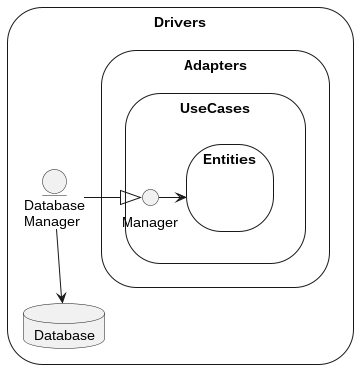
\includegraphics[width=0.9\textwidth]{../img/clean}
            \end{center}
        \end{column}
    \end{columns}


\end{frame}
%------------------------------------------------
